% !TEX root = MAIN.tex

\section{LXS - ESAIL System Test Suite}
\label{chapter:caseStudies:LXS}

\subsection{Overview of the case study}

\INDEX{ESAIL} is a microsatellite developed by LXS in a PPP with ESA and ExactEarth. 
The Payload is an AIS Receiver for ship- and vessel-detection from space, and the satellite weight at launch will be approximately 115kg. The satellite payload also enables advanced raw data handling and RF-Spectrum sampling for Ground processing.

\begin{figure}[h]
	\centering
    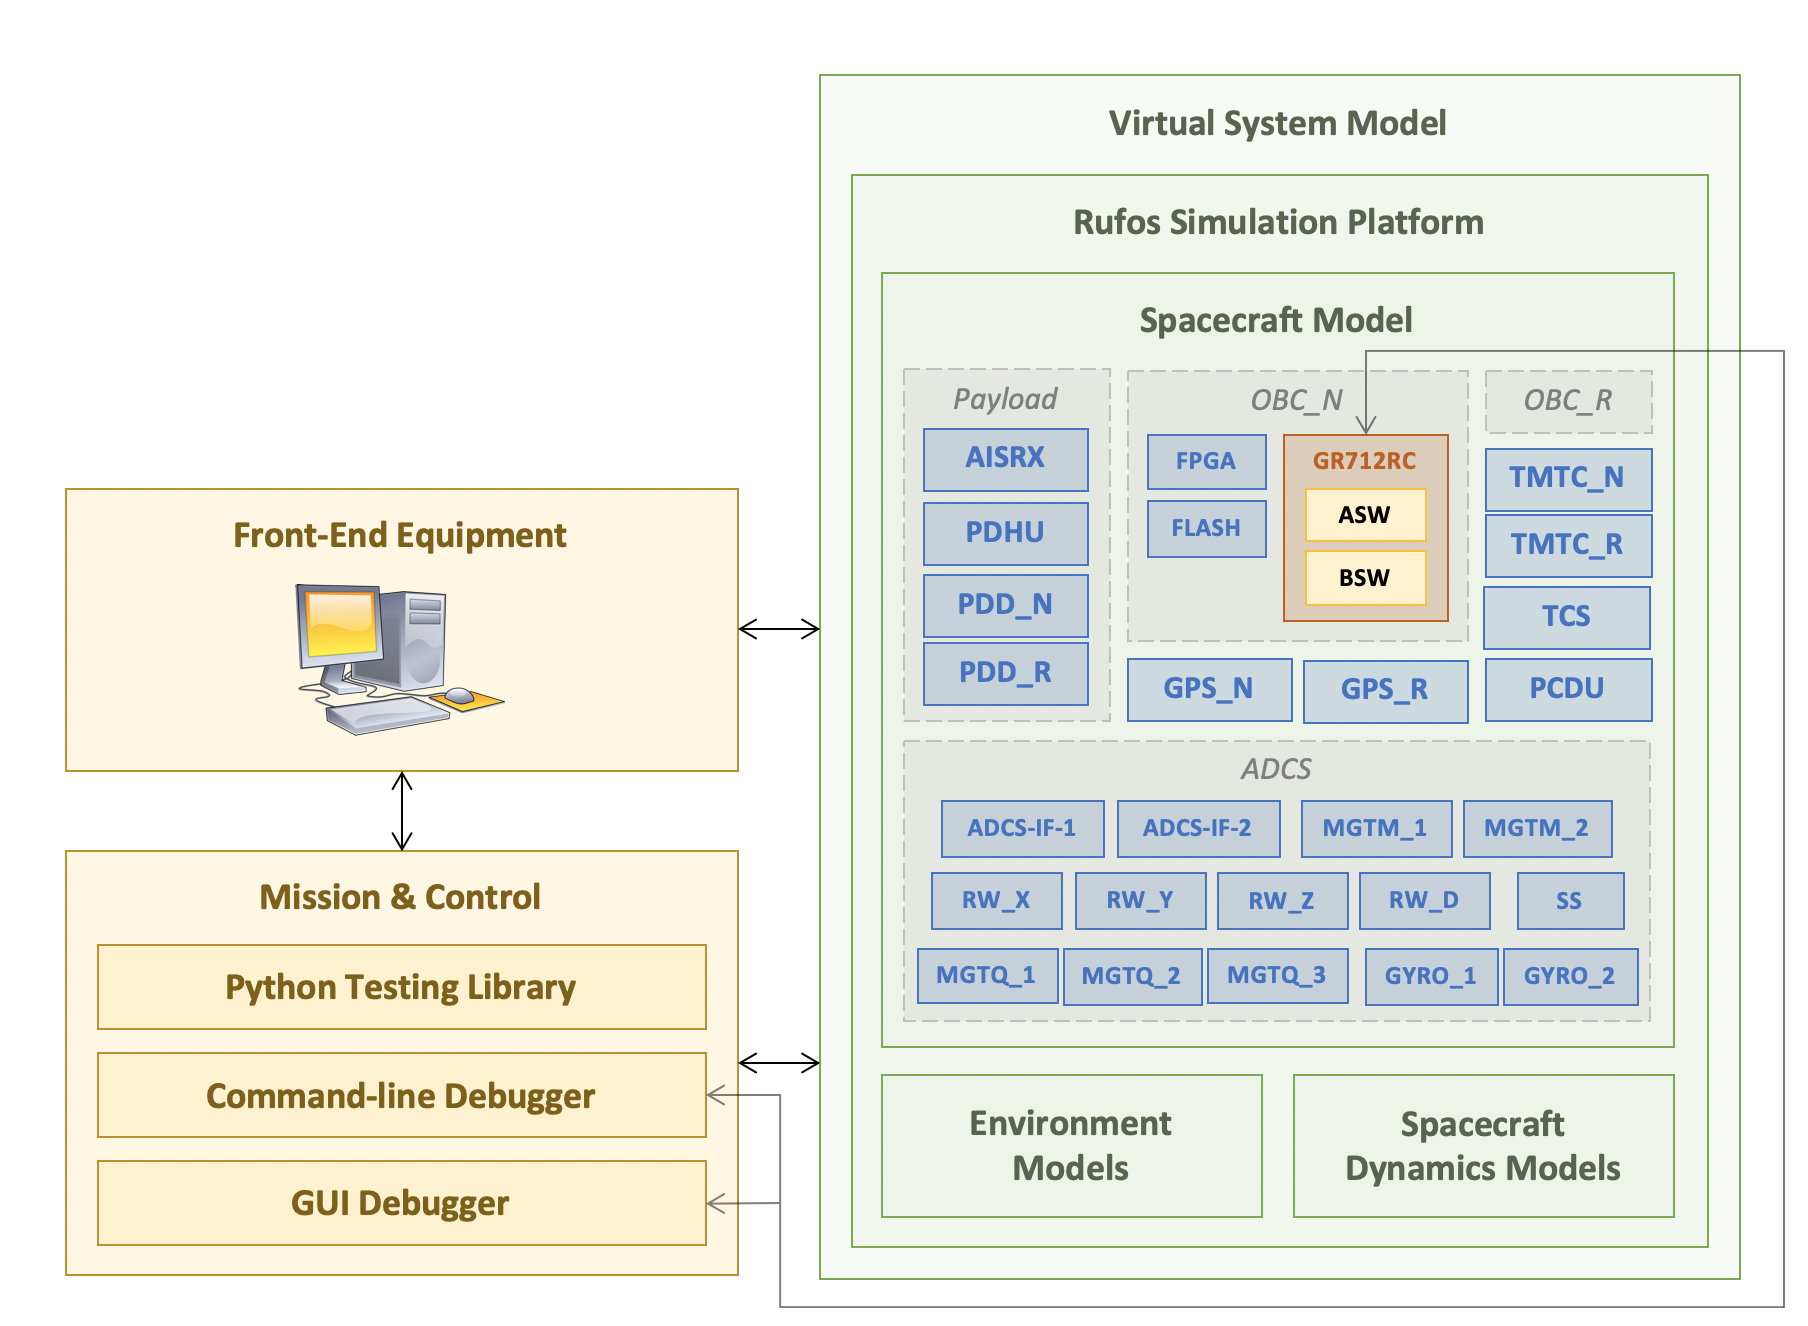
\includegraphics[width=0.7\textwidth]{images/esail}
    \caption{ESAIL system testing environment.}
    \label{fig:esail_case_study}
\end{figure}
 
The \INDEX{SVF simulator} has been used for functional validation of the ESAIL CSW (see Figure~\ref{fig:esail_case_study}). The SVF is indeed one of the main testing tools used in satellite projects. The SVF simulator can be seen as a testing facility that presents also its own dedicated test suite to ensure the correctness of the SVF models and assembly to avoid later misunderstanding of the expected behaviours of the satellite CSW. 
In the context of the FAQAS project we consider the system test suite for the validation of the CSW, which are implemented using the SVF as the driving tool.
%Therefore, the SVF Simulator enables the evaluation of the FAQAS framework against two test suites: (1) the Test Suite of the SVF Simulator that validates the Simulator itself, (2) the system tests for the validation of CSW, which are implemented using the SVF as the driving tool.

%Details about ESAIL are provided in the document \emph{FAQAS-LXS-MAN-001\_1- SVF Software Installation and User Manual} uploaded on Alfresco.

ESAIL is the largest case study system in FAQAS, the software consists of 924 source files with a total size of 187\,116 LOC. The system test suite consists of 121 python test scripts with a total of 384 sub-test cases. 
\MREVISION{C-P-22}{The system test suite takes up to 10 hours to finish its execution; the total execution time may be different and depends on the processing power of the computer where the SVF is being executed.}

\subsection{ESAIL System Test Suite Environment}

Because of the objectives of the project, we will need to execute a large number of mutants. Even if strategies for simplifying and reducing the number of mutants are designed (see Section~1.2.4 from D2), there is a need for an infrastructure for running several mutant executions on parallel, which particularly applies for the ESAIL System Test Suite (e.g., the test suite execution time is high).

The University of Luxembourg provides a High-Performance Computing platform for academic purposes\footnote{https://hpc.uni.lu}.
The HPC has a computing capacity of 690 nodes, totaling 11\,280 computing cores, and a storage capacity of 8\,742 TB.

Given that ESAIL runs on a simulator (i.e., SVF), which is compute-intensive, and that resources of the UL HPC are shared between multiple jobs, non-deterministic behaviors are seldom observed (e.g., test cases fail because of lack of resources).

In view of the code-driven mutation testing process, where the quality of a test suite is assessed by checking if an injected fault is detected by the existing test cases, we need a test suite with a deterministic behavior, that is, if a test case fails it exclusively depends if we have introduced an artificial fault (i.e., a code mutation), and not because of the running environment.

To ensure that a mutant has been actually killed when executing the ESAIL System Suite on the UL HPC, we propose to execute a test case up to 10 times. If for any of this 10 executions the mutant is not killed, we consider it a live mutant. Otherwise, if it fails 10 times, we consider it a killed mutant.



\subsection{LXS - ESAIL Unit Test Suite}
\label{chapter:caseStudies:LXS:Unit}



The unit test suite of ESAIL will be considered for the evaluation of the final FAQAS toolset. 
%For example, it is a possible case to be used for an independent use of the FAQAS framework by LXS engineers. The ESAIL unit test suite is used mainly to test critical functionalities of ESAIL components. The ESAIL unit test suite has been provided to ESA; however, the mutation testing activity might concern a subset of them. Indeed, evaluating with mutation testing a set of test cases that are known for covering only a subset of the features of the system might be of little usefulness. 
%%The set of test cases and functions to be tested will be provided along with the description of the achieved results at the end of WP3.
To assess the quality of the ESAIL unit test suite we will analyze the same ESAIL sub-system defined in Section~\ref{lxs:esail:system:codeDriven}, and thus, we will target the same set of mutants. Since the ESAIL Unit Test Suite has been implemented by LXS to cover scenarios hard to cover with a full simulation (consequently, it covers a limited portion of the code), we will use the ESAIL Unit Test Suite to provide a complementary analysis to the one given by the system test suite.
Precisely, we rely on the ESAIL unit test suite to evaluate if mutation analysis results can be combined (see Section~\ref{sec:exp:thr}). 


%Regarding code coverage, the ESAIL system test suite reports 67,022 out of 74,155 lines of code being covered (i.e., 90.38% statement coverage). 



\REVOCT{C-P-6}{In the ESAIL development context, the unit test suite is used to exercise critical functions hard to exercise with the system test suites. For this reason, the unit test suite covers only a portion of the code (i.e., 46.5\% statement coverage). MASS applies mutation analysis only to code that is covered by the test suite, for this reason, since we rely on the unit test suite only to evaluate the combination of multiple test suites, only the code coverage of the system test suite is relevant (i.e., we do not mutate lines exercised by the unit test suite only).} 

%In our empirical evaluation, we rely on the ESAIL unit test suite to evaluate if mutation analysis results can be combined (see Section~\ref{sec:exp:thr}). 
%In the ESAIL development context, the unit test suite is used to exercise critical functions hard to exercise with the system test suites. For this reason, the unit test suite covers only a portion of the code (i.e., 46.5\% statement coverage). 
%MASS applies mutation analysis only to code that is covered by the test suite, for this reason, since we rely on the unit test suite only to evaluate the combination of multiple test suites, only the code coverage of the system test suite is relevant (i.e., we do not mutate lines exercised by the unit test suite only).